\documentclass{article}
\usepackage{graphics} 
\usepackage{hyperref}
\usepackage{fixltx2e}
\usepackage{amssymb}
\usepackage{tikz}

\author{Kevin Zollicoffer}
\title{Regression\\Lesson 1b}
\date{10/14/2013}

\usepackage{Sweave}
\begin{document}
\maketitle
%\tableofcontents
\Sconcordance{concordance:Assignment1b.tex:Assignment1b.Rnw:%
1 11 1 1 0 14 1 1 2 4 0 1 2 4 1 1 2 1 0 2 1 4 0 1 2 4 1 1 2 1 0 4 1 4 0 %
1 2 4 1 1 2 1 0 1 1 22 0 1 2 34 1 1 2 4 0 1 2 1 1 1 2 1 0 1 1 6 0 1 2 2 %
1 1 2 1 0 1 1 22 0 2 2 1 0 1 1 22 0 1 2 23 1 1 2 1 0 1 1 4 0 2 2 1 0 1 %
1 4 0 1 2 11 1}


\section*{Introduction}
Regression assignment 1b using R. 
\\
\\
The complete source for this assigment is available on Github:
\\
\\
\url{https://github.com/zollie/PASS-Regression-Assignment1b}

\section*{Problem 2.3}
\begin{Schunk}
\begin{Sinput}
> elec <- read.csv("~/R/PASS/Regression/Assignment1b/electricity.csv")
\end{Sinput}
\end{Schunk}

\subsection*{a}
GDP should be the predictor vairable with Electricity should be the response vairable. b\textsubscript{1} would be positive under the claim that electricity consumption increases in response to increases in GDP.

\subsection*{b}
\begin{Schunk}
\begin{Sinput}
> plot(elec$Gdp, elec$Elec)
> model <- lm(elec$Elec ~ elec$Gdp)
> lines(sort(elec$Gdp), fitted(model)[order(elec$Gdp)])
\end{Sinput}
\end{Schunk}
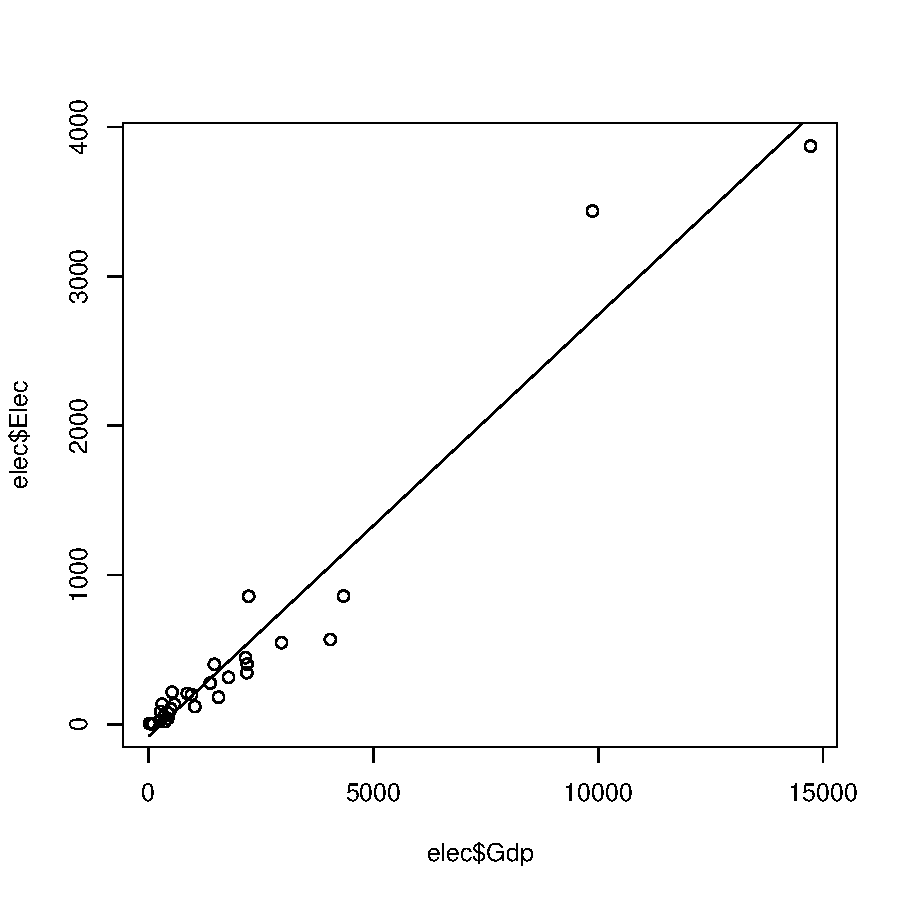
\includegraphics{Assignment1b-002}

\noindent
There is a clearly a positive relationship between GDP and electrictiy consumption in a country. There are 2 outliers skewing the results to the right, and perhaps overestimating the slope of the resultant regression line. This increases the standard error of the model. It also bunches the non-outlier data points toward the lower left of the model inhibiting interpretation of the model. 

\subsection*{c}
\begin{Schunk}
\begin{Sinput}
> max2 <- order(elec$Gdp,decreasing=T)[1:2]
> elec2 <- elec[-max2,]
> plot(elec2$Gdp, elec2$Elec)
> model2 <- lm(elec2$Elec ~ elec2$Gdp)
> lines(sort(elec2$Gdp), fitted(model2)[order(elec2$Gdp)])
\end{Sinput}
\end{Schunk}
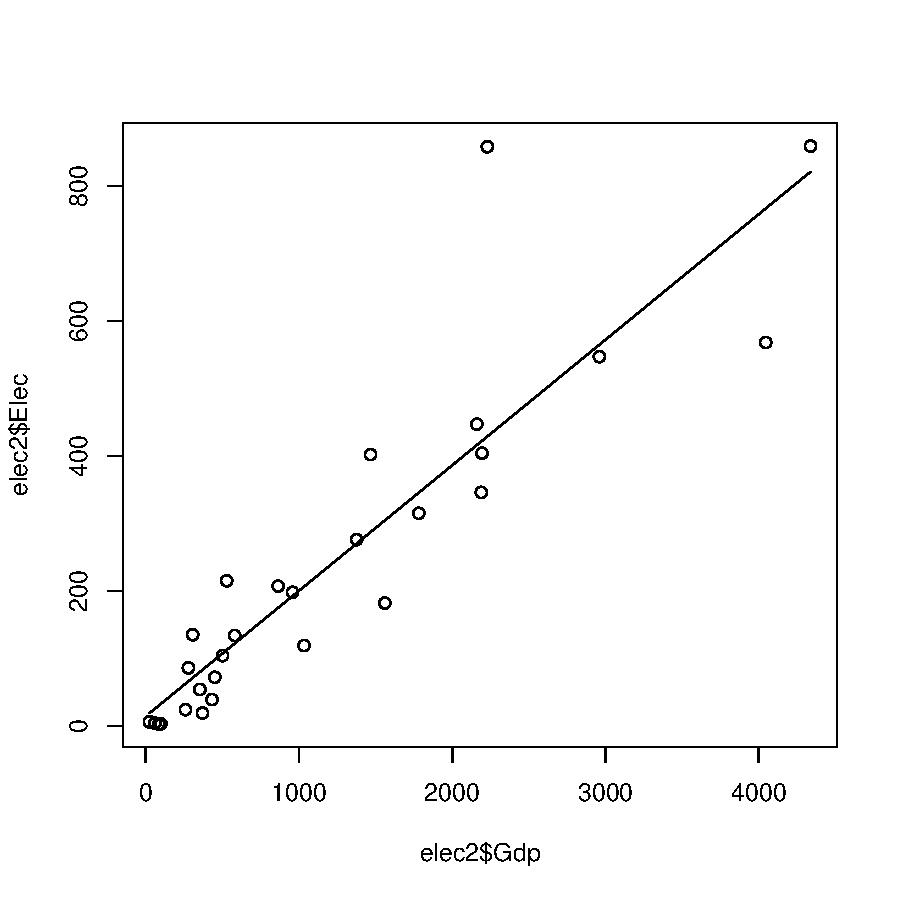
\includegraphics{Assignment1b-003}

\noindent
With the 2 outliers removed, the standard error is apprently decreased and the obersvations appear more tightly correlated about the regression line (taking into account the scale of the X/Y axes). 

\subsection*{d}
\begin{Schunk}
\begin{Sinput}
> options(scipen=999) # disable scientific notation
> summary(model2)
\end{Sinput}
\begin{Soutput}
Call:
lm(formula = elec2$Elec ~ elec2$Gdp)

Residuals:
    Min      1Q  Median      3Q     Max 
-198.69  -32.61  -18.01   22.78  429.21 

Coefficients:
            Estimate Std. Error t value        Pr(>|t|)    
(Intercept) 14.27579   29.11331    0.49           0.628    
elec2$Gdp    0.18596    0.01752   10.62 0.0000000000601 ***
---
Signif. codes:  0 ‘***’ 0.001 ‘**’ 0.01 ‘*’ 0.05 ‘.’ 0.1 ‘ ’ 1

Residual standard error: 107 on 26 degrees of freedom
Multiple R-squared:  0.8126,	Adjusted R-squared:  0.8054 
F-statistic: 112.7 on 1 and 26 DF,  p-value: 0.00000000006009
\end{Soutput}
\end{Schunk}

\subsubsection*{Hypotheis Test}
\noindent
$H_{0} = b_{1} = 0
\\
H_{a} = b_{1} > 0
\\
b_{1}\:t-stat=10.62
\\
b_{1}\:p-value=.00000000601  
$ 

\noindent
\newline
t-distribution upper tail signifigance level for 5\% (1-.05) confidence and 26 degrees of freedom = 1.706 

\paragraph{Hypothesis Test Result}
\noindent
\\
\\
$b_{1}\:t-stat=10.62 > 1.706 \therefore reject\:H_{0}$
\\
\\
alternatively
\\
\\
$b_{1}\:p-value=.00000000601 < .005 \therefore reject\:H_{0}$
\noindent
\\\\
An elec2\$Gdp slope of zero seems inplausible. The sample data favor a positive slope at 5\% confidence level. 

\subsection*{e}
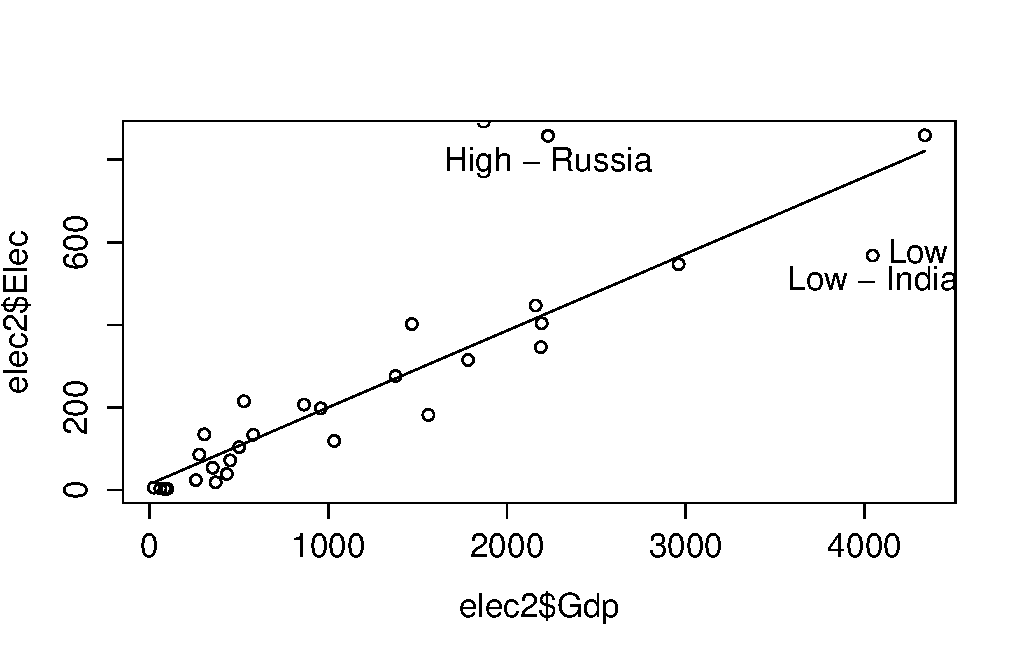
\includegraphics[width=0.98\textwidth]{HighLow.pdf}

\section*{2.5}
\begin{Schunk}
\begin{Sinput}
> cars2 <- read.csv("~/R/PASS/Regression/Assignment1b/cars2.csv")
\end{Sinput}
\end{Schunk}

\subsection*{a}
\begin{Schunk}
\begin{Sinput}
> cars2[["Cgphm"]] <- 100/cars2$Cmpg
> mean(cars2$Cgphm)
\end{Sinput}
\begin{Soutput}
[1] 4.613156
\end{Soutput}
\end{Schunk}

\subsection*{b}
\subsubsection*{Regression using Eng as the predictor}
\begin{Schunk}
\begin{Sinput}
> model_eng <- lm(Cgphm ~ Eng, data=cars2)
> summary(model_eng)
\end{Sinput}
\begin{Soutput}
Call:
lm(formula = Cgphm ~ Eng, data = cars2)

Residuals:
     Min       1Q   Median       3Q      Max 
-0.61401 -0.22593 -0.04419  0.15520  1.32962 

Coefficients:
            Estimate Std. Error t value            Pr(>|t|)    
(Intercept)   2.5894     0.1026   25.24 <0.0000000000000002 ***
Eng           0.8183     0.0397   20.61 <0.0000000000000002 ***
---
Signif. codes:  0 ‘***’ 0.001 ‘**’ 0.01 ‘*’ 0.05 ‘.’ 0.1 ‘ ’ 1

Residual standard error: 0.3351 on 125 degrees of freedom
Multiple R-squared:  0.7726,	Adjusted R-squared:  0.7708 
F-statistic: 424.8 on 1 and 125 DF,  p-value: < 0.00000000000000022
\end{Soutput}
\end{Schunk}
\subsubsection*{Regression using Vol as the predictor}
\begin{Schunk}
\begin{Sinput}
> model_vol <- lm(Cgphm ~ Vol, data=cars2)
> summary(model_vol)
\end{Sinput}
\begin{Soutput}
Call:
lm(formula = Cgphm ~ Vol, data = cars2)

Residuals:
    Min      1Q  Median      3Q     Max 
-1.2039 -0.4521 -0.1067  0.3734  2.3482 

Coefficients:
            Estimate Std. Error t value    Pr(>|t|)    
(Intercept)   1.8760     0.5337   3.515    0.000613 ***
Vol           2.5010     0.4849   5.157 0.000000953 ***
---
Signif. codes:  0 ‘***’ 0.001 ‘**’ 0.01 ‘*’ 0.05 ‘.’ 0.1 ‘ ’ 1

Residual standard error: 0.6382 on 125 degrees of freedom
Multiple R-squared:  0.1755,	Adjusted R-squared:  0.1689 
F-statistic:  26.6 on 1 and 125 DF,  p-value: 0.0000009527
\end{Soutput}
\end{Schunk}

\subsubsection*{Residual standard error evaluation}
For the linear regression model using Eng as the predictor $s=.3351$
\\\\
For the linear regression model using Vol as the predictor $s=.6382$
\\\\
$.3351 < .6382 \therefore  $ when considering s, the model using predictor Eng is preferable

\subsubsection*{Coefficient of determination - R\textsuperscript{2}}
For the linear regression model using Eng as the predictor $R^2=.7726$
\\\\
For the linear regression model using Vol as the predictor $R^2=.1755$
\\\\
$.7726 > .1755 \therefore  $ when considering $R^2$, the model using predictor Eng is preferable. Moreover, .1755 is significantly < 1, therefore the model using Vol as the predictor is highly questionable. 

\subsubsection*{The p-value of $b_{1}$}
For the linear regression model using Eng as the predictor the p-value of Eng =0.0000000000000002
\\\\
For the linear regression model using Vol as the predictor the p-value of Vol=0.0000009527
\\\\
$.0000000000000002 < .0000009527 \therefore  $ when considering the statistical significance of $b_{1}$, the model using predictor Eng is preferable. 

\subsubsection*{Visual Interpretation}
\paragraph*{Eng}
\begin{Schunk}
\begin{Sinput}
> plot(cars2$Eng, cars2$Cgphm)
> lines(sort(cars2$Eng), fitted(model_eng)[order (cars2$Eng)])
\end{Sinput}
\end{Schunk}
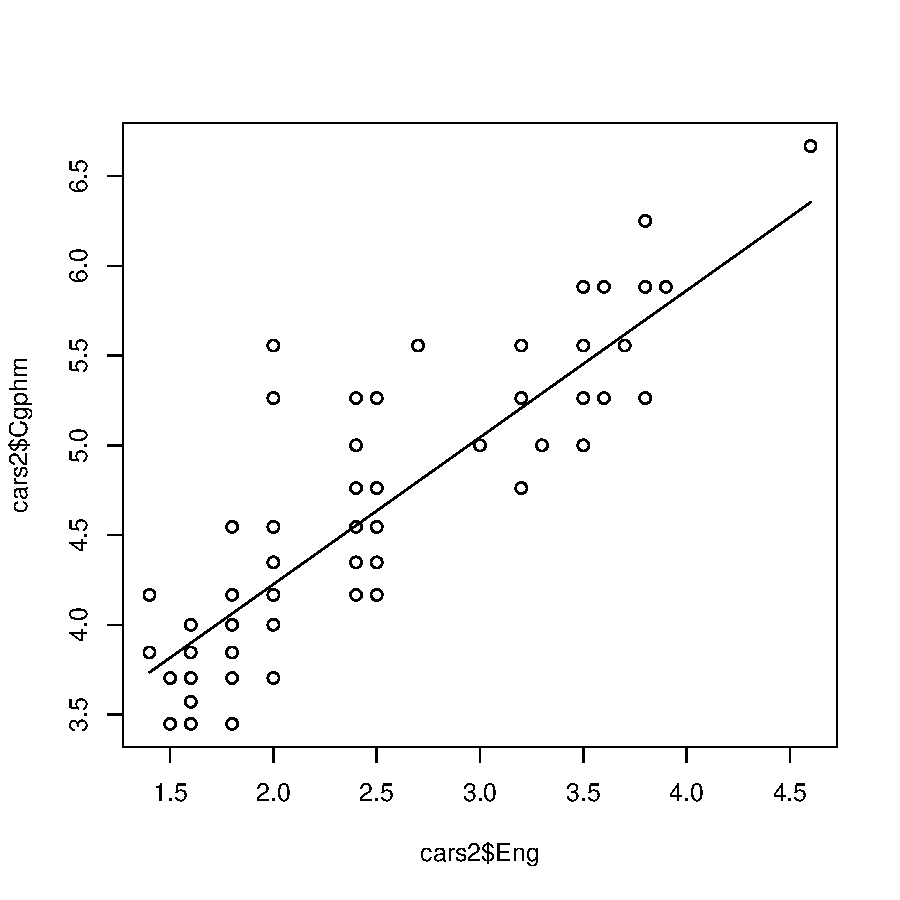
\includegraphics{Assignment1b-009}
\paragraph*{Vol}
\begin{Schunk}
\begin{Sinput}
> plot(cars2$Vol, cars2$Cgphm)
> lines(sort(cars2$Vol), fitted(model_vol)[order (cars2$Vol)])
\end{Sinput}
\end{Schunk}
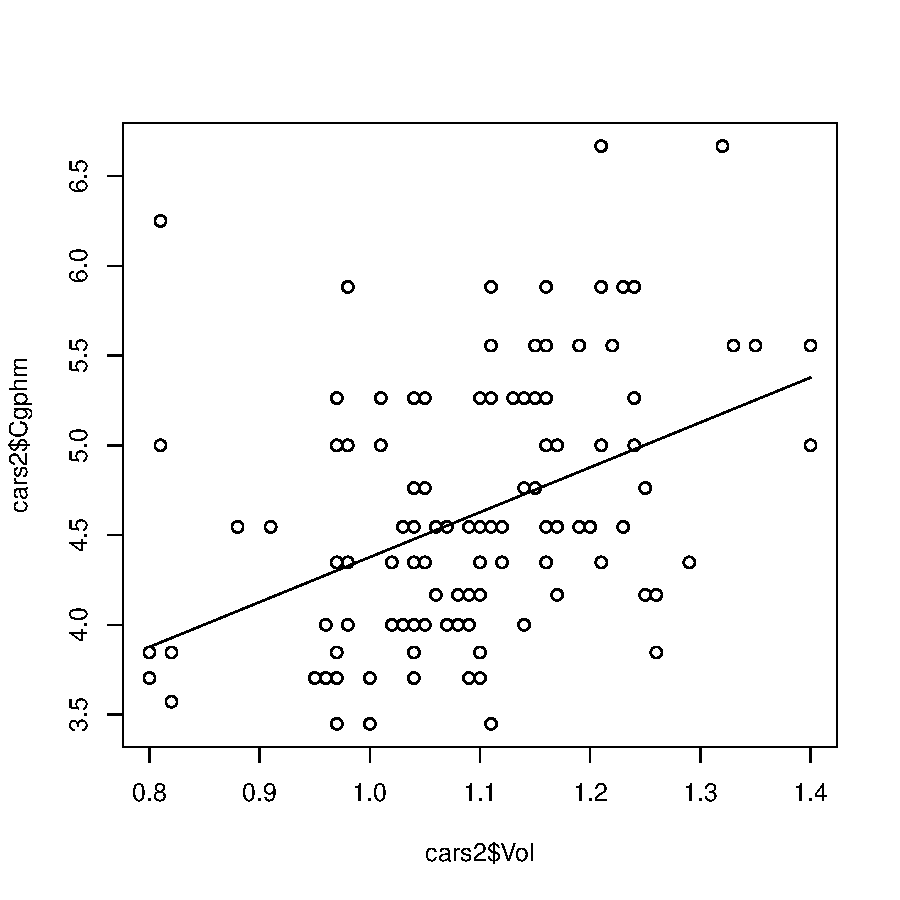
\includegraphics{Assignment1b-010}

\subsection*{}
Visually the plot of Eng is more tightly correlated around the regression line and the slope of the regression line exhibits more lift. Using Eng as the predictor is preferable over using Vol as the predicotr for this linear regression excercise. 

\subsection*{c}
Using Eng as the predictor for the cars2 data was reccomended. As shown above $s=.3351$ for this model. 

\noindent
\\
It can be shown that approximately 95\% of the observed Y-values lie within approximately $\pm$ 2s, therefore it can be said that with 95\% confidence our future predictions of Y using this linear regression model will fall within $\pm 2s$. That is, we have a 95\% confidence interval of $((X).8183 \pm .6702)$ given an observation of Eng=X.  

\end{document}
